\section{Overview}
In this work, we will define the label categories forged as 1 $(y=1)$ and genuine as 0 $(y=0)$ for handwritten signatures, and the input reference signature image is defined as $R \in \mathbb{R}^{H\times W\times 1}$ and the query signature image is defined as $Q \in \mathbb{R}^{H\times W\times 1}$.

\begin{figure}[htbp]
  \begin{center}
      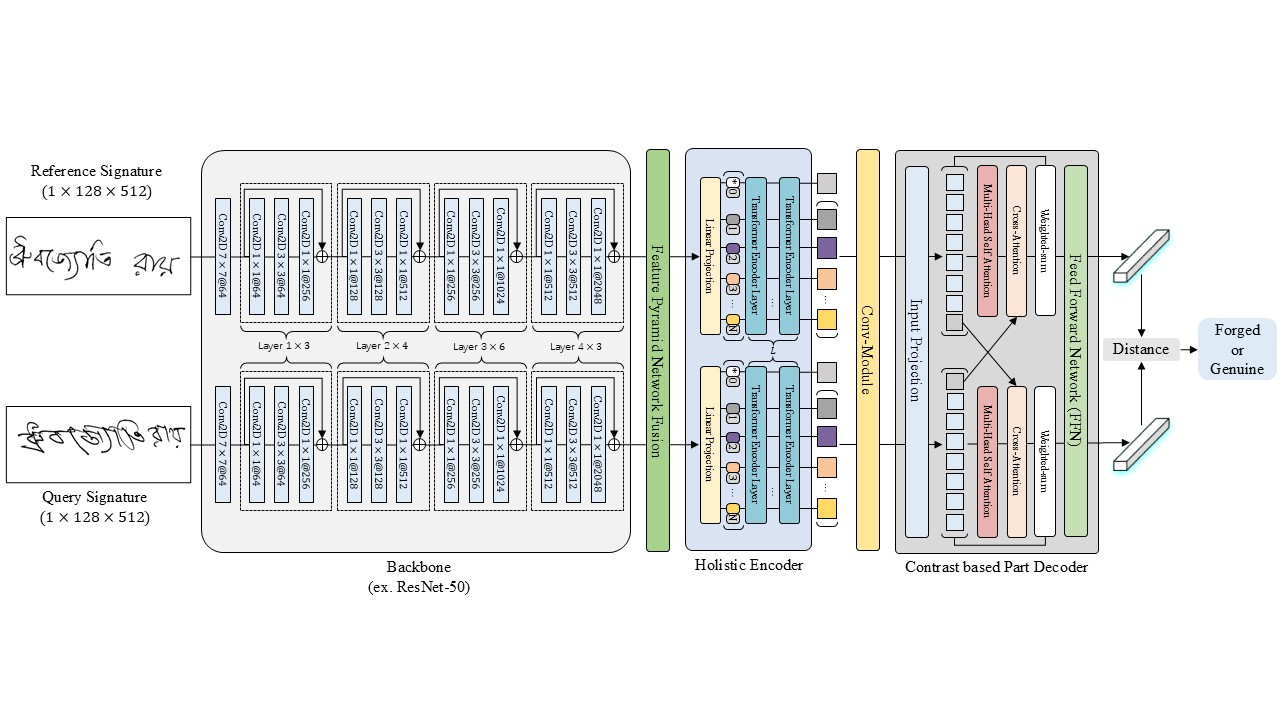
\includegraphics[scale=0.46]{figure/osvtf.jpg}
  \end{center}
  \caption{OSVTF structure Detail}
  \label{fig:osvtf}
\end{figure}

The architecture of the proposed Offline Signature Verification TransFormer (OSVTF) model for multi-scale feature fusion is shown in Fig. \ref{fig:osvtf}, which consists of five parts, namely, Backbone ($\mathcal{B}$), FPN Fusion ($\mathcal{F}$), Holistic Encoder ($\mathcal{H}$), and Conv-Module ($\mathcal{C}$), Contrast based Part Decoder ($\mathcal{P}$) five parts. In the model we will input a pair of signature image samples $\mathbf{I}_r$ and $\mathbf{I}_q$, the initial input image goes through Backbone with shared weights (ResNet-50 \cite{14} is used as an example in Fig. \ref{fig:osvtf}) to get the multi-scale feature map set $\mathcal{B}(\mathbf{I}_r),\mathcal{B}(\mathbf{I}_q)$, and then the different scale feature maps are fused through FPN Fusion module, and the output of multi-scale fusion feature maps $\mathbf{F}_r^\mathcal{F},\mathbf{F}_q^\mathcal{F}$. Then it enters the Holistic Encoder with shared weights to get the holistic flat features $f_r^\mathcal{H},f_q^\mathcal{H}$ and patch embeddings $\boldsymbol{x}_r^\mathcal{H}=[x_r^{\mathcal{H}_1 }, \cdots, x_r^{\mathcal{H}_N} ]$ and $\boldsymbol{x}_q^\mathcal{H} = [ x_q^{\mathcal{H}_1}, \cdots, x_q^{\mathcal{H}_N} ]$. To further integrate the feature maps, the above patch embeddings are reshaped to a 2D shape, and its outputs $\mathbf{F}_r^\mathcal{C}, \mathbf{F}_q^\mathcal{C}$ are obtained after the Convolutional Module (Conv-Module) with shared weights, and they will go directly to the Contrast based Part Decoder to obtain the cross-attention contrast part flat features $f_r^\mathcal{P},f_q^\mathcal{P}$. In the final prediction stage, Global Average Pooling (GAP) operation is performed on $\mathbf{F}_r^\mathcal{F},\mathbf{F}_q^\mathcal{F}$ and $\mathbf{F}_r^\mathcal{C},\mathbf{F}_q^\mathcal{C}$ to obtain the multiscale fusion flat features $f_r^\mathcal{F},f_q^\mathcal{F}$ and convolution flat features $f_r^\mathcal{C},f_q^\mathcal{C}$. The total feature vector $f_r=[f_r^\mathcal{F},f_r^\mathcal{H},f_r^\mathcal{C},f_r^\mathcal{P} ]$ and $f_q=[f_q^\mathcal{F},f_q^\mathcal{H},f_q^\mathcal{C},f_q^\mathcal{P} ]$ of the OSVTF are obtained by splicing all the flat features, and the judgment of whether $\mathbf{I}_q$ is forged or not will be made based on $f_r$ and $f_q$. Next, Backbone, FPN Fusion, Holistic Encoder, Conv-Module and Contrast based Part Decoder structures will be analyzed in depth.

\section{Backbone}

In the Backbone section an architecture of CNN will be adopted that discards Average Global Pooling and Fully Connected Layers in the output section.Most of the CNN architecture consists of a convolutional layer in the input section and four defined convolutional layers, as shown in Fig. 3 for example in ResNet-50 \cite{14}, where each layer consists of a number of bottleneck blocks. A single bottleneck block consists of two convolutional 2D layers with convolutional kernels of ($1\times 1 \to 3\times 3 \to 1\times 1$), and this arrangement mainly has the following purposes: 1. Reduce the feature dimensions to achieve the purpose of improving the computational efficiency; 2. The intermediate $3\times 3$ convolution extracts the local spatial features such as strokes, edges, etc., in the lower dimensional space has the ability to maintain the sensory field while reducing the redundancy, and this reduces the number of channels before expanding to the input, and then the number of channels is expanded to the input, and the number of channels is reduced. This first reduces the number of expression channels and then expands to the input expression channels to find better feature learning parameters in the bottomleneck, which has a better feature abstraction and expression ability; 3. In the actual operation, it can be paired with the identity skip connection to quickly propagate the gradient to avoid gradient disappearance, and at the same time, such a design makes the number of intermediate parameters and the burden of computation greatly reduced, and it can stack more layers. At the same time, this design can greatly reduce the number of intermediate parameters and computational burden, and can stack more layers, such as ResNet-101, to promote the training of deeper networks; 4. This modular design has the advantage of easy fine-tuning of the convolutional parameters, and the number of intermediate channels can be adjusted according to the environment, so as to control the balance of performance and efficiency. In addition, ResNet series network introduces residual connection, which solves the problem of missing features after deep convolutional operation of the image. Residual connection is introduced in each bottomleneck block, which accumulates the feature map of the input part with the output of the bottomleneck, which can reduce the problem of feature loss after a certain number of convolutional layer operations to a certain extent.

Assume that the input feature map $ \mathbf{I} \in \mathbb{ R }^{ H\times W\times C } $ of the convolutional layer, the output feature map $\boldsymbol{z} \in \mathbb{ R }^{ H'\times W'\times C' }$, the convolutional kernel size of the convolutional 2D layer $K\times K$ (the convolutional kernel weight $ \tilde{\mathbf{W}} \in \mathbb{ R }^{ K\times K\times C\times C' } $, the padding $\tilde{P}$, the step size $\tilde{S}$, and the bias term $\tilde{b}$. For the $c'$-th output channel of the feature map, the pixel point with spatial location $(i,j)$ is calculated as eq. \ref{eq1}.

\begin{equation}
\label{eq1}
  \boldsymbol{z}(i, j, c') = \sum^{C'}_{c=1} \sum^K_{u=1} \sum^K_{v=1} = \tilde{\mathbf{W}}_{u, v, c, c'} \cdot \mathbf{I}(i\cdot \tilde{S}+u-\tilde{P}, j\cdot \tilde{S}+v - \tilde{P}, c) + \tilde{\mathbf{b}}_{c'}
\end{equation}

In addition, in each bottleneck block, except for the last $1\times 1$ convolutional 2D layer which is followed only by the BatchNorm (BN) \cite{16} operation, each convolutional 2D layer will be followed immediately by the BN and ReLU activation function \cite{29} operation (Conv2D$\to$BN$\to$ReLU), and the spatial location $(i,j,c')$ after the BN and ReLU activation function is the pixel point values are as eq. \ref{eq2}.

\begin{equation}
\label{eq2}
  \hat{\boldsymbol{z}}(i, j, c') = \max \left( 0, \gamma_c \frac{\boldsymbol{z}(c', i, j) - \mu'_c}{\sqrt{\sigma^2_{c'}+\epsilon}}+\beta_{c'} \right)
\end{equation}

Where $\mu,\sigma^2$ are the mean and variance of the feature statistics of the $c'$ channel plane in the batch multi-channel feature maps output from the convolutional 2D layer, and $\gamma, \beta$ are the learnable scaling and translation parameters. This shows that the idea of the BN operation is to normalize a certain batch of data, which has the effect of improving the convergence speed when training the model parameters. In each bottomleneck block operation, a cumulative residual operation is performed on the feature maps after three convolutional 2D operations, i.e., the feature maps input to the bottomleneck block are added to the feature maps output from the three convolutional 2D operations, which are then passed to the next bottomleneck block. At the same time, each layer of the backbone operation will be followed by a downsampling operation as a way to reduce the redundant features on the multi-channel feature map, which will be taken as Max Pooling 2D in order to equate the downsampling operation \cite{14}. The above residual linking approach can ensure that the feature map retains certain original image features after the convolution operation, so the ResNet family of networks is most suitable as the backbone of the depth model to extract the image multi-channel feature map.

The backbone is taken mainly to extract the image multi-scale feature maps, so the different scale feature maps of each layer except the input convolutional layer are included in the final output as eq. \ref{eq3}.

\begin{equation}
\label{eq3}
  \mathcal{B}(\mathbf{I}) = \{ \mathbf{F}^{\mathcal{B}(1)}, \mathbf{F}^{\mathcal{B}(2)}, \mathbf{F}^{\mathcal{B}(3)}, \mathbf{F}^{\mathcal{B}(4)} \}
\end{equation}

where the multi-channel feature map $\mathbf{F}^\mathcal{B}(i) \in \mathbb{R}^{\frac{H}{2^{i+1}} \times \frac{W}{2^{i+1}} \times \frac{C}{2^{i-1}}},(i=1,2,3,4)$ for each scale, H,W,C denote the width, height and the number of channels of the output feature maps of layer 1, and $C=256$ when the backbone is ResNet-50), and each layer of the feature map has a twofold relationship between the channels and dimensions.

\section{FPN Fusion}

In order to be able to effectively utilize the multi-scale feature maps extracted by backbone, the Feature Pyramid Network Fusion (FPN Fusion) module is used in order to fuse feature maps at different scales, which adopts the model architecture of FPN-Style \cite{23}, as shown in Figure \ref{fig:fpn}.

\begin{figure}[htbp]
  \begin{center}
      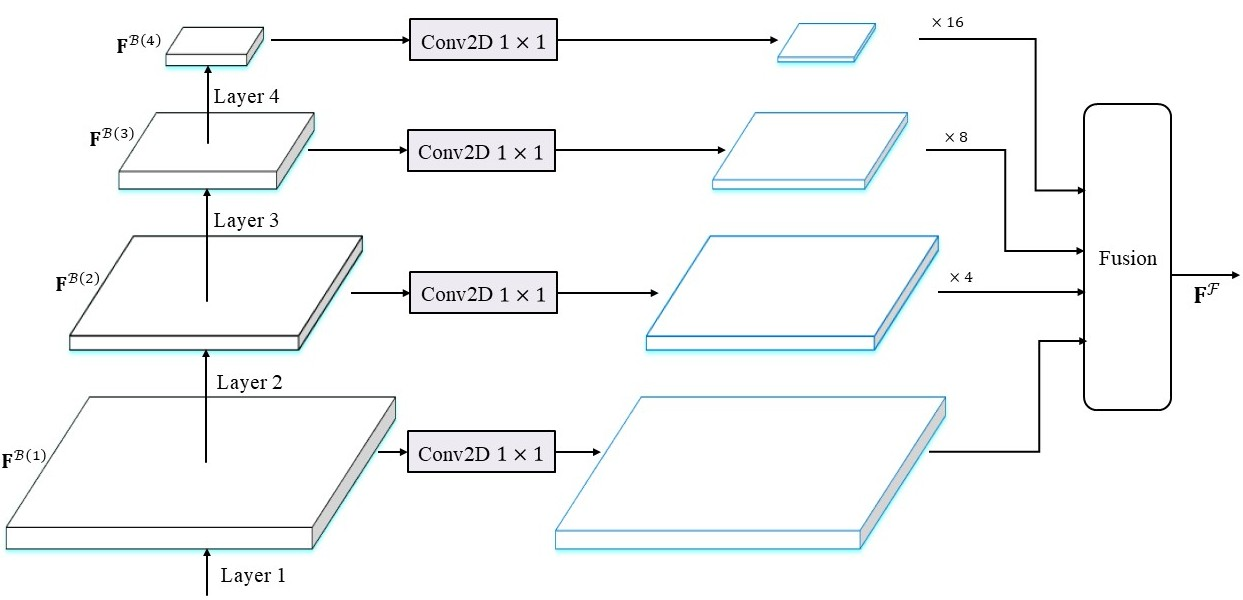
\includegraphics[scale=0.45]{figure/fpn.jpg}
  \end{center}
  \caption{FPN Fusion module structure}
  \label{fig:fpn}
\end{figure}

Where the bottom-up process is the process of backbone inference to obtain different scales of feature maps. In bottom-down, for each layer of feature maps, a convolutional 2D layer with a convolutional kernel of $1\times 1$ will be taken for mapping, which maps the feature maps with different number of channels at each scale to the same feature dimensions, and achieves the operation of dimensionality reduction to a certain extent, so as to accelerate the speed of model inference. At the same time, $\mathbf{F}^{\mathcal{B}(2)} ,\mathbf{F}^{\mathcal{B}(3)} ,\mathbf{F}^{\mathcal{B}(4)}$ are up-sampled to increase the size to the same size as $\mathbf{F}^{\mathcal{B}(1)}$, and then fused according to the fusion method in order to get the multi-scale fusion feature map. Bilinear interpolation \cite{18} is adopted in the up-sampling process, for the lth layer feature map up-sampling output $\mathbf{F}^{\mathcal{B}(l)}$, the value of spatial location $(i',j',c)$ is calculated as eq. \ref{eq4}.

\begin{equation}
\label{eq4}
  \begin{aligned}
    \mbox{Up}(\mathbf{F}^{\mathcal{B}(l)})(i', j', c) &= (1-\delta_i)(1-\delta_j)\cdot \mathbf{F}^{\mathcal{B}(l)}(i, j, c)\\
    &+\delta_i(1-\delta_j)\cdot \mathbf{F}^{\mathcal{B}(l)}(i+1, j, c) \\
    &+(1-\delta_i)\delta_j\cdot \mathbf{F}^{\mathcal{B}(l)}(i, j+1, c) \\
    &+\delta_i \delta_j \cdot \mathbf{F}^{\mathcal{B}(l)}(i+1, j+1, c)
  \end{aligned}
\end{equation}

where $\delta_i=\frac{i'}{s_i} - \lfloor \frac{i'}{s_i} \rfloor, \delta_j = \frac{j'}{s_j} - \lfloor \frac{j'}{s_j} \rfloor$ denote fractional portions of the value in the direction of the width and the height, $s_i,s_j$ denote the magnification $(s_i = s_j = 2)$, and $\lfloor \cdot \rfloor$ denotes the value of the integer part. This up-sampling method can well preserve the original feature ground structure while introducing a smooth transition as shown in Fig. \ref{fig:bilinear}. 

\begin{figure}[htbp]
  \centering
  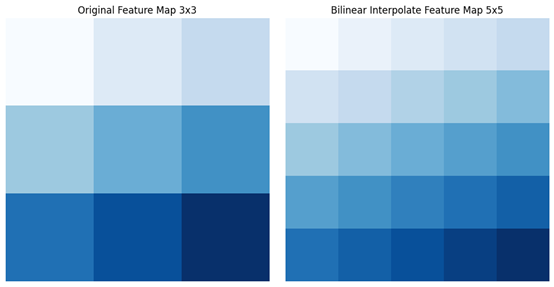
\includegraphics[scale=0.8]{figure/bilinear.png}
  \caption{Bilinear interpolation example}
  \label{fig:bilinear}
\end{figure}

Each up-sampled pixel point will be weighted according to the original feature map pixel points, which not only retains the structural scale of the original feature map, but at the same time makes the transition between pixel points smoother, and to a certain extent, it can reflect the effect of different scales on the image feature points, for example, the features of a certain stroke will be enlarged.

After each scale feature map is sampled on the ground by bilinear interpolation, it will be fused according to three ways: accumulation, weighted average, and channel splicing. The first way is the traditional FPN-Style approach, which directly performs the accumulation operation on the downscaled multi-scale feature maps directly, similar to the residual link mentioned above. The design idea of the second way is to be able to ensure that the signature images of different scenarios can have a certain learning ability, by setting the proportion of weights to be able to pay more attention to the features of a certain scale, and the default is to take all equal weights. The third way is to splice in the channel dimension, followed by a convolutional kernel $1\times 1$ convolutional 2D operation, this method can maximize the retention of all scales of features, but may lead to the model computational overhead is too large, resulting in slower convergence of the model.

After fusing the multi-scale feature map, it will finally go through a convolutional 2D layer with a convolutional kernel $3\times 3$ to smooth out the checkerboard artifacts brought about by the up-sampling process, and finally output the multi-scale fused feature map $\mathbf{F}^\mathcal{F} = \mathcal{F}(\mathcal{B}(\mathbf{I})) \in \mathbb{R}^{\frac{H}{4}\times \frac{W}{4}\times C}$.

\section{Holistic Encoder}

\begin{figure}[H]
  \begin{center}
      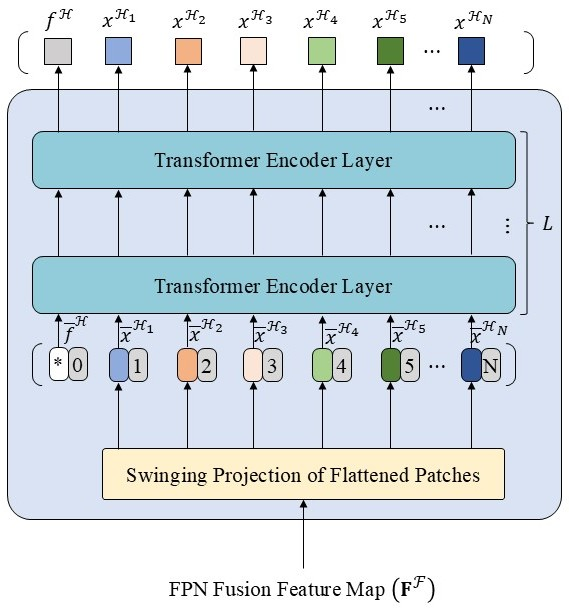
\includegraphics[scale=0.6]{figure/encoder.jpg}
  \end{center}
  \caption{Holistic Encoder structure}
  \label{fig:encoder}
\end{figure}

The Holistic Encoder is designed with reference to Vision Transformer (ViT) \cite{4} The architecture is shown in Fig. 6. swing embeddings \cite{24} are adopted in the input stage instead of the previous chunking operation, where chunking and mapping are performed on the input multiscale fusion feature maps according to the set window size $P\times P$ and step size S , the patch embeddings are obtained and then flattened to be used as feature vectors $[\overline{x}^{\mathcal{H}_1},\overline{x}^{\mathcal{H}_2},\cdots ,\overline{x}^{\mathcal{H}_N}] \in \mathbb{R}^{N\times D}$, where D denotes the number of mapped feature dimensions, and the vector length, $N$, is computed as eq. \ref{eq5}.


\begin{equation}
\label{eq5}
  N=\lfloor \frac{H/4-P+S}{S}\rfloor \times \lfloor \frac{W/4-P+S}{S}\rfloor
\end{equation}

Splicing a learnable weight $\overline{f}^{\mathcal{H}}\in \mathbb{R}^D$ defined as a class token in swing embeddings, i.e., the feature vector of the input Transformer Encoder Layer is $\overline{\boldsymbol{x}}^\mathcal{H}=[\overline{f}^\mathcal{H},\overline{x}^{\mathcal{H}_1},\overline{x}^{\mathcal{H}_2},\cdots ,\overline{x}^{\mathcal{H}_N} ] \in \mathbb{R}^{(N+1)\times D}$. Due to the flattening operation performed on the feature map, positional embeddings \cite{36} need to be accumulated on the feature vectors as a way to make the feature vectors contain information about their positions on the multiscale fused feature map.

After swing embeddings, the feature vector $\overline{\boldsymbol{x}}^\mathcal{H}$ enters the Transformer Encoder Layer for attention feature computation. Where Transformer Encoder Layer is formed by $L$ stacks as shown in Fig. \ref{fig:mhsa}.

\begin{figure}[H]
  \begin{center}
      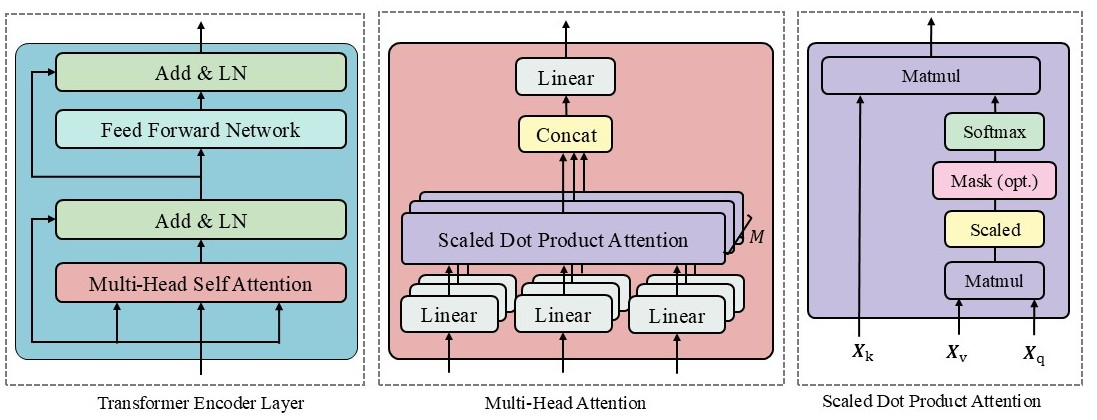
\includegraphics[scale=0.55]{figure/mhsa.jpg}
  \end{center}
  \caption{Transformer Encoder Layer structure}
  \label{fig:mhsa}
\end{figure}

Each Transformer Encoder Layer consists of a Multi-Head Self Attention $\to$ Add \& LN and Feed Forward Network $\to$ Add \& LN, where Add \& LN denotes residual linking and LayerNormalization (LN) \cite{1}. The input feature vectors first enter Multi-Head Self Attention (MHSA) in order to perform the computation of the attention mechanism, which is essentially Multi-Head Attention (MHA) except that the sources before the mapping of $\boldsymbol{X}_\text{q} \in \mathbb{R}^{N\times d_q}$ and $\boldsymbol{X}_\text{k}, \boldsymbol{X}_\text{v} \in \mathbb{R}^{N\times d_k }$ in the operations are The same, i.e., the input feature vectors will be simultaneously entered into the linear mapping layer of each head for dimensionality reduction, thus generating the query vector $\boldsymbol{X}_\text{q}$, the key vector $\boldsymbol{X}_\text{k}$, the value vector $X_v$, and $d_q = d_k$. where the attention mechanism is divided into multiple head computations in order to conserve the computational resources, and the feature vectors will be entered into the three linear layers of the $M$ heads in order to be dimensionality reduced for mapping, thus achieving the attention computation in parallel, and the final splice and linear layer mapping will input vectors with the same feature dimensions, so the output vector shape of MHSA is the same as the input vector shape. The attention feature vectors of each head in MHSA are computed by taking scaled dot product attention \cite{36} with the following eq. \ref{eq6}.

\begin{equation}
\label{eq6}
  \text{Attn}(\boldsymbol{X}_\text{v}, \boldsymbol{X}_\text{k}, \boldsymbol{X}_\text{v}) = \text{Softmax} \left( \frac{\boldsymbol{X}_\text{q}\boldsymbol{X}_\text{k}^\mathrm{T}}{\sqrt{d_k}} \right)\cdot \boldsymbol{X}_\text{v}
\end{equation}

In this case, there is a soft query relationship between $\boldsymbol{X}_\text{q}, \boldsymbol{X}_\text{k}$ and $\boldsymbol{X}_\text{v}$. Instead of selecting a specific key-value pair for each query, all key-values are weighted and averaged, and the weights are computed by the similarity between $\boldsymbol{X}_\text{q}$ and $\boldsymbol{X}_\text{k}$. each feature token of $\boldsymbol{X}_\text{q}$ establishes a relevance distribution, i.e., a Softmax \cite{37} of attention weights, based on which the values of $\boldsymbol{X}_\text{v}$ are weighted and fused. The advantage of this mechanism is that it can focus on multiple relevant tokens at the same time, which enables the model to more fully model the contextual information, for example, the $(i, j)$ position of attention weight indicates the weight of $i$-th position of $\boldsymbol{X}_\text{q}$ on the $j$-th position of $\boldsymbol{X}_\text{k}$, the larger the value of this weight, the stronger the contextual relationship of the query at the $i$-th position to the key at $j$-th position, and conversely the smaller the value, the relationship is very small. According to this attention weight, multiplying $\boldsymbol{X}_\text{v}$ again will further amplify the features in the place where the attention weight of its own vector is high, and the attention information will be included between tokens, so as to achieve that each token owns its own global information, and can more effectively utilize the important features and ignore the useless features, and will more effectively pay attention to the part of the brush strokes in the image of the handwritten signature, ignoring the blank part. The resulting MHSA output of a single Transformer Encoder Layer is as eq. \ref{eq7}.

\begin{equation}
\label{eq7}
\text{MHSA}(\overline{\boldsymbol{x}}^\mathcal{H},\mathbf{T},\mathbf{L}) =
\begin{bmatrix}
  \text{Attn}(\overline{\boldsymbol{x}}^\mathcal{H} \mathbf{T}_{1,1},\overline{\boldsymbol{x}}^\mathcal{H} \mathbf{T}_{1,2},\overline{\boldsymbol{x}}^\mathcal{H} \mathbf{T}_{1,3}) \\
  \text{Attn}(\overline{\boldsymbol{x}}^\mathcal{H} \mathbf{T}_{2,1},\overline{\boldsymbol{x}}^\mathcal{H} \mathbf{T}_{2,2},\overline{\boldsymbol{x}}^\mathcal{H} \mathbf{T}_{2,3}) \\
  \cdots \\
  \text{Attn}(\overline{\boldsymbol{x}}^\mathcal{H} \mathbf{T}_{m,1},\overline{\boldsymbol{x}}^\mathcal{H} \mathbf{T}_{m,2},\overline{\boldsymbol{x}}^\mathcal{H} \mathbf{T}_{m,3}) \\
\end{bmatrix}^{\mathrm{T}}
\cdot \mathbf{L} 
\end{equation}

where $\mathbf{T}_l \in \mathbb{R}^{M\times 3\times d_k\times d_k' }$ denotes the linear mapping layer weights in the input phase of the MHSA, $\mathbf{L} \in \mathbb{R}^{d_k\times d_k' }$ denotes the weights of the final linear mapping layer in the MHSA, and $d_k'$ denotes the number of feature dimensions of each head $\boldsymbol{X}_\text{q}, \boldsymbol{X}_\text{k}$ and $\boldsymbol{X}_\text{v}$, and thus must satisfy $d_k=M\times d_k'$.

Matrix multiplication with larger dimensions is performed in the MHSA section, and in order to reduce the risk of gradient explosion or vanishing, and also to reduce the missing information of the original feature vectors, a residual link and an LN layer follow immediately after the MHSA.The main role of the LN layer is to normalize the feature vectors at each position, thus speeding up the convergence of the model as well as improving the model stability. Unlike the mean and variance of the BN, the mean and variance of the LN are derived from the current feature dimensions on which they are calculated as eq. \ref{eq8}.

\begin{equation}
\label{eq8}
\begin{aligned}
  \mu &= \frac{1}{d_k}\sum^{d_k}_d \text{MHSA}(\overline{\boldsymbol{x}}^\mathcal{H}, \mathbf{T}, \mathbf{L})_d \\
  \sigma^2 &= \frac{1}{d_k}\sum^{d_k}_d \left( \text{MHSA}(\overline{\boldsymbol{x}}^\mathcal{H}, \mathbf{T}, \mathbf{L})_d - \mu \right)^2
\end{aligned}
\end{equation}

where $\text{MHSA}(\overline{\boldsymbol{x}}^\mathcal{H},\mathbf{T},\mathbf{L})_d$ denotes the dth feature dimension of the MHSA output feature vector. The subsequent normalization operation is the same as in the BN layer, and the entire MHSA$\to$Add \& LN output is computed as eq. \ref{eq9}.

\begin{equation}
\label{eq9}
  \hat{\text{MHSA}}(\overline{\boldsymbol{x}}^\mathcal{H}, \mathbf{T}, \mathbf{L}) = \gamma \cdot \left( \frac{\text{MHSA}(\overline{\boldsymbol{x}}^\mathcal{H}, \mathbf{T}, \mathbf{L}) - \mu}{\sqrt{\sigma^2+\epsilon}} + \mathcal{E}_{l-1} \right) + \beta
\end{equation}

Where $\mathcal{E}_{l-1}$ denotes the output of the previous Transformer Encoder Layer, if $l=1$, then $\mathcal{E}_{l-1}=\overline{\boldsymbol{x}}^\mathcal{H}$. After the attention computation, Feed Forward Network (FFN) is introduced to enhance the overall model to model the complex patterns \cite{8}, and the whole FFN is computed as eq. \ref{eq10}:

\begin{equation}
\label{eq10}
  \text{FFN}(\hat{\text{MHSA}}(\overline{\boldsymbol{x}}^\mathcal{H}, \mathbf{T}, \mathbf{L})) = \mathcal{G}(\hat{\text{MHSA}}(\overline{\boldsymbol{x}}^\mathcal{H}, \mathbf{T}, \mathbf{L})\mathbf{W}_1 + \mathbf{b}_1)\mathbf{W}_2 + \mathbf{b}_2
\end{equation}

Where $\mathbf{W}_1\in \mathbb{R}^{D\times d_{ff}}, b_1\in \mathbb{R}^{d_{ff}}$ denotes the weight and bias of the first linear layer in the FFN, and $\mathbf{W}_2\in \mathbb{R}^{d_{ff}\times D}, \mathbf{b}_2\in \mathbb{R}^D$ denotes the weight and bias of the second prior layer in the FFN, $\mathcal{G}$ denotes the GeLU function \cite{15}. the GeLU function and the ReLU function act similarly as the activation function that performs the nonlinear transformation. The entire FFN is a nonlinear transformation of the model, which complements the global interaction mechanism of Attention to jointly build a powerful context-aware representation. Subsequently followed by Add \& LN to supplement the feature information and accelerate the model convergence, each subsequent layer of Transformer Encoder Layer is a stacking effect to deepen the Attention weight of the feature vectors, and the output of the whole Holistic Encoder is $\{f^\mathcal{H}, \boldsymbol{x}^\mathcal{H} \} = \mathcal{H}(F^\mathcal{F}),f^H\in \mathbb{R}^D,x^\mathcal{H} \in R^{N\times D}$.

\section{Conv-Module}

The image features are subjected to feature learning by Holistic Encoder capturing the relative position information of the elements in the sequence, but it has the limitation of learning absolute position information. The signature verification task needs to be accurate to the stroke position information (e.g., stroke order, local structural differences), so after this in order to enhance some small portion of the image features, the output $\boldsymbol{x}^\mathcal{H}$ of the patch token of the Holistic Encoder is rearranged, and the flattened token is reconverted into a 2D shape $\mathbf{F}^\mathcal{H} \in \mathbb{R}^{h\times w\times D}$ to perform a convolution operation, where $h = \lfloor \frac{H/4-P+S}{S}\rfloor,w = \lfloor \frac{W/4-P+S}{S}\rfloor $. This module introduces the convolution operation to reprocess the patch features output from the Transformer encoder to enhance the position-awareness. In the Conv-Module architecture, the Conv design of TransOSV \cite{41} is referenced, and the number of output channels of the intermediate convolutional 2D layer is adjusted to increase the downsampling operation according to the style of previous CNNs, as shown in Table \ref{tab:conv}.


\begin{table}[htbp]
\caption{Conv-Module layers information}  
\begin{center}
\begin{tabu} to 0.8\textwidth{X[3, c]X[3, c]X[3, c]}  
%0.8\textwidth   为设置表格宽度  
%X[c]      表示这一列居中,所占比例为1,相当于X[1,c]  
%X[3,c]   表示这一列居中,所占比例为3,这列的宽度是X[c]列的3倍  
\toprule
Layer & Kernel Size & Output feature map\\
\midrule
Conv2D + ReLU & $3\times 3$ & $h\times w\times d_\mathcal{C}$ \\ 
Conv2D + ReLU & $3\times 3$ & $h\times w\times d_\mathcal{C}$ \\ 
Max Pooling 2D & $2\times 2$ & $\frac{h}{2}\times \frac{w}{2}\times d_\mathcal{C}$ \\ 
Conv2D + ReLU & $3\times 3$ & $\frac{h}{2}\times \frac{w}{2}\times \frac{d_\mathcal{C}}{2}$ \\ 
Conv2D + ReLU & $3\times 3$ & $\frac{h}{2}\times \frac{w}{2}\times \frac{d_\mathcal{C}}{2}$ \\ 
Conv2D + ReLU & $3\times 3$ & $\frac{h}{4}\times \frac{w}{4}\times \frac{d_\mathcal{C}}{2}$ \\ 
\bottomrule
\end{tabu}
\end{center}
\label{tab:conv}
\end{table}

Different from the traditional CNN with gradually more channels, the overall downsampling operation thinking is adopted here, and certain downsampling operations are performed on the patch features to abstractly express the local features of the feature map on the basis of integrating the local detail features, with the purpose of enhancing the generalization ability and robustness of the model. This operation is added on the basis of backbone and FPN Fusion to further strengthen the model's ability to perceive the local features of the image, strengthen the focus on the key local regions of the signature, and filter the background interference at the same time. In the Conv-Module module, each Conv2D layer operation is the same as the Conv2D layer operation in backbone, which takes the combination of Conv2D+ReLU, and after two Conv2D+ReLUs a downsampling operation, i.e., Max Pooling 2D operation, will be performed to integrate the feature maps and eliminate the non-important parts of the features to integrate and eliminate non-important parts of the feature map and enhance feature expressiveness.

In the model training process, the output $\mathbf{F}^\mathcal{C} = \mathcal{C}(\mathbf{F}^\mathcal{H} ) \in \mathbb{R}^{h'\times w'\times d_C' }$ of the Conv-Module will undergo a Global Average Pooling (GAP) operation while entering the Contrast based Part Decoder to globally sample the feature maps of the output of the Conv-Module. The feature maps of the Conv-Module are globally sampled to obtain a flat local convolutional feature $f^\mathcal{C}$ to complete the corresponding feature extraction in the training and inference process.

\section{Contrast based Part Decoder}

\begin{figure}[H]
  \centering
      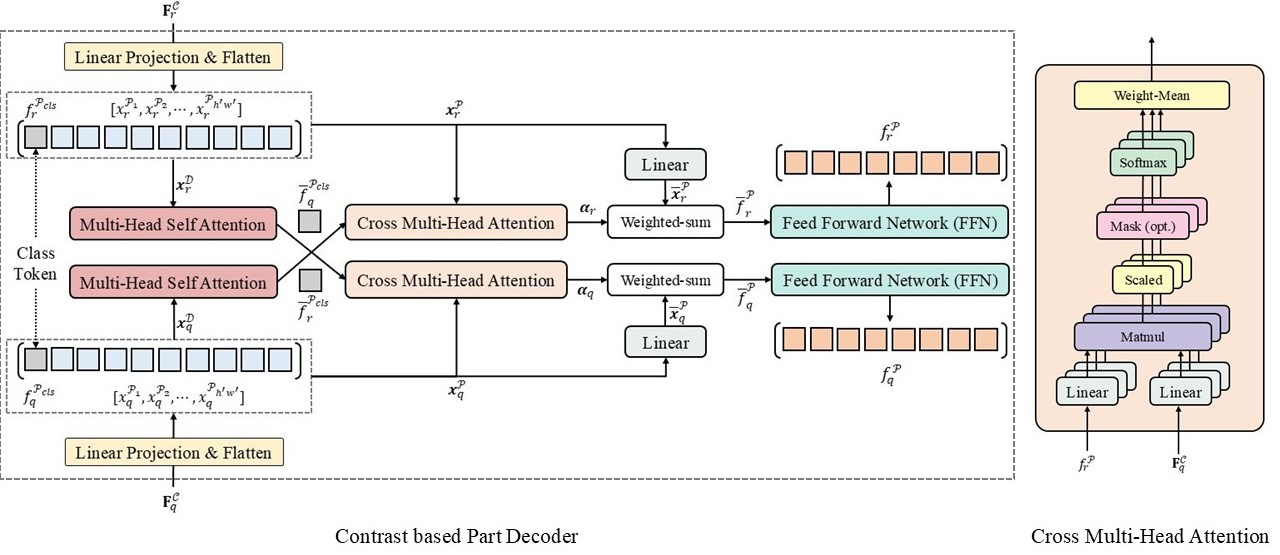
\includegraphics[scale=0.45]{figure/decoder.jpg}
  \caption{Contrast based Part Decoder structure}
  \label{fig:decoder}
\end{figure}

This part is an improvement on TransOSV's Contrast based Part Decoder \cite{41} for parallel computation of Cross-Attention, which references the multi-head attention computation mechanism of MHSA in Holistic Encoder. Similar to the Holistic Encoder part, the feature maps of references and query are mapped to the $d_\mathcal{P}$ feature dimension in the input phase, followed by flattening and addition of a learnable weight $f_r^{\mathcal{P}_{cls}},f_q^{\mathcal{P}_{cls}} \in \mathbb{R}^D$, also defined as a class token, i.e., the input part is obtained as a pair of flattened feature map vectors $\boldsymbol{x}_r^\mathcal{P} = [f_r^{\mathcal{P}_{cls}}, x_r^{\mathcal{P}_1},\cdots ,x_r^{\mathcal{P}_{h' w' }} ]$, $\boldsymbol{x}_q^\mathcal{P}=[f_q^{\mathcal{P}_{cls}},x_q^{\mathcal{P}_1},\cdots,x_q^{\mathcal{P}_{h'w'} } ] \in \mathbb{R}^{h' \times w' \times (D+1)}$. Subsequently, MHSA operations are performed on $\boldsymbol{x}_r^\mathcal{P},\boldsymbol{x}_q^\mathcal{P}$ to take out the class token $\overline{f}_r^{\mathcal{P}_{cls}},\overline{f}_q^{\mathcal{P}_{cls}} \in \mathbb{R}^D$ of their respective output eigenvectors as the query matrix cross-input Cross Multi-Head Attention (CMHA).The structure of CMHA is shown in Figure 8-b shown, differs from MHA in that only the query matrix and key matrix are generated to compute their cross-attention weights $\boldsymbol{\alpha}_r,\boldsymbol{\alpha}_q$, and the final concat is replaced with a weighted average to handle the attention weights of multiple heads. For a single CMHA the output cross-attention weight $\boldsymbol{\alpha}$ is calculated as eq. \ref{eq11}.

\begin{equation}
\label{eq11}
  \boldsymbol{\alpha}= \frac{1}{M}\sum^M_{m=1} \text{Softmax}\left( \frac{\boldsymbol{X}_\text{q}\mathbf{T}^\mathcal{P}_{m, 1}\cdot (\boldsymbol{X}_\text{k}\mathbf{T}^\mathcal{P}_{m, 2})^\mathrm{T} }{\sqrt{d_\mathcal{P}'}} \right)
\end{equation}

where $\boldsymbol{X}_\text{q},\boldsymbol{X}_k$ denote the input query and key vectors, $\mathbf{T}^\mathcal{P} \in \mathbb{R}^{M\times 2\times D\times d_k′}$ denotes the linear mapping layer weights of the input part of the CMHA. The resulting $\boldsymbol{\alpha}_r,\boldsymbol{\alpha}_q$ computation process is as eq. \ref{eq12}.

\begin{equation}
\label{eq12}
\begin{aligned}
  \boldsymbol{\alpha}_r = \frac{1}{M}\sum^M_{m=1} \text{Softmax}\left( \frac{\overline{f}_q^{\mathcal{P}_{cls}}\mathbf{T}^\mathcal{P}_{m, 1}\cdot (\boldsymbol{x}_r^\mathcal{P}\mathbf{T}^\mathcal{P}_{m, 2})^\mathrm{T} }{\sqrt{d_\mathcal{P}'}} \right) \\
  \boldsymbol{\alpha}_q = \frac{1}{M}\sum^M_{m=1} \text{Softmax}\left( \frac{\overline{f}_r^{\mathcal{P}_{cls}}\mathbf{T}^\mathcal{P}_{m, 1}\cdot (\boldsymbol{x}_q^\mathcal{P}\mathbf{T}^\mathcal{P}_{m, 2})^\mathrm{T} }{\sqrt{d_\mathcal{P}'}} \right) \\
\end{aligned}
\end{equation}

Perform a weight-sum operation on the attention weights and the mapped flat feature vector $\overline{\boldsymbol{x}}_r^\mathcal{P},\overline{\boldsymbol{x}}_r^\mathcal{P}\in \mathbb{R}^{h'\times w'\times d_\mathcal{P}}$, and fuse to generate the flat feature $\overline{f}_r^P,\overline{f}_q^P\in \mathbb{R}^{d_P}$ with cross-attention weights. Its after FFN to get the flat feature $\overline{f}_r^\mathcal{P},\overline{f}_q^\mathcal{P}\in \mathbb{R}^{d_P}$ of cross attention of decoder, the whole computation process is as eq. \ref{eq13}.

\begin{equation}
\label{eq13}
  \{f_r^\mathcal{P},f_q^\mathcal{P},\boldsymbol{\alpha}_r,\boldsymbol{\alpha}_q \}=\mathcal{P}(F_r^\mathcal{C},F_q^\mathcal{C} )
\end{equation}

This Contrast based Part Decoder, which is similar to the structure of Transformer Decoder \cite{36}, facilitates the generation of local feature information that distinguishes between genuine and forged signatures, and emphasizes the feature relationship between a pair of data samples, enhancing the model's learning of the features between a pair of data in a sample. During the training process, the output cross-attention weights $\boldsymbol{\alpha}_r,\boldsymbol{\alpha}_q$ are computed with sparsity loss to force the distribution of cross-attention weights to be centralized, avoiding averaging in order to fail to pay attention to the sensitive part of forged signatures.

\section{Loss Funcion}

\subsection{Euclidean Distance}

OSVTF is a model architecture similar to twin networks, this style emphasizes that the model is a two-flow form of shared weights and the overall purpose is to compare the gap between the two, so it will be based on the similarity of the input two features in order to design the loss function. In this work, Euclidean Distance \cite{5} will be taken in order to be used as a similarity calculation for a pair of feature samples, assuming that a pair of features $f_r,f_q$ is input and the formula for calculating the distance between them is as eq. \ref{eq14}.

\begin{equation}
\label{eq14}
  \mathcal{D}(f_r, f_q) = ||f_r - f_q||_2=\sqrt{\sum_{d=1}(f^{(d)}_r - f^{(d)}_q)^2}
\end{equation}

\subsection{Focal Contrast Loss}

In the handwritten signature sample data processing stage, the handwritten signature of the writer will be paired with the pairing operation that will not be repeated between the two, for example, the BHSig-B \cite{3} dataset contains a total of 100 writers' handwritten signature images, in which each writer owns 24 genuine signature images ($y=0$) and 30 forged signature images ($y=1$), the genuine signature images are used as the reference signature, forged signature and real signature together as query signature, which will generate 276 pairs of positive samples and 720 pairs of negative samples. Thus each writer has a total of 996 data sample pairs, in which the ratio between positive and negative sample pairs is not close to 50:50, so the number of positive and negative samples is not balanced and belongs to the category of hard samples \cite{33}. 

The loss function of similarity of comparison samples used for binary classification in earlier algorithms and models is Contrast Loss \cite{10}, which is calculated as eq. \ref{eq15}.

\begin{equation}
\label{eq15}
  \mathcal{L}_c (f_r,f_q ) = (1 - y)\cdot \mathcal{D}(f_r,f_q)^2 + y\cdot \max⁡(m - \mathcal{D}(f_r,f_q),0)^2 
\end{equation}

Where $m$ denotes the boundary value, i.e., the distance that forged samples should be kept at least. For the sample pair of $y=0$, it is directly used as the loss value to make the model parameter learning on the real sample pairs of features more similar; on the contrary $y=1$, if the feature distance between the reference and query is less than $m$, $(m - \mathcal{D}(f_r,f_q ))^2$ is used as the loss value to make the model for the forged signature pairs of features is not less than $m$. However, this kind of loss can't be dynamically emphasized on the hard samples and is prone to model parameter overfitting problems. In order to reduce the risk of overfitting, a boundary value is also introduced for the genuine sample pairs to reduce the unnecessary contraction between the genuine pairs, i.e., the Double-Margin loss \cite{25} is calculated as eq. \ref{eq16}.

\begin{equation}
\label{eq16}
\begin{aligned}
  \mathcal{L}_{dm} (f_r,f_q ) &= (1-y)\cdot \max(\mathcal{D}(f_r,f_q )-n,0)^2 \\
  &+ y\cdot \max⁡(m-\mathcal{D}(f_r,f_q),0)^2
\end{aligned}  
\end{equation}

where the two boundary values m>n, penalize the case where the distance exceeds n for the genuine sample pairs, and promote the case where the distance is greater than m for the forged sample pairs. Although double margin optimizes the problem of easy overfitting by contrast loss to a certain extent, in the case of two pairs of sample data $\{r,q_1 \},\{r,q_2\}$ and $y=1$ In the case, the distance between the two sample pairs is calculated by OSVTF, if $\mathcal{D}(f_r,f_{q_1}) >> \mathcal{D}(f_r,f_{q_2}) > n $, then the loss function should give a greater loss to ${r,q_1}$, but $\mathcal{L}_{dm}$ will treat the two sample pairs equally, and the notion of dynamic weighting is introduced in TransOSV, named Focal Contrast Loss \cite{41}, which is calculated as eq. \ref{eq17}.

\begin{equation}
\label{eq17}
\begin{aligned}
  \mathcal{L}_{fc}(f_r,f_q ) &= (1 - y)\cdot \sigma(\overline{K}(\mathcal{D}(f_r,f_q )-\alpha_1 ))\cdot \max⁡(\mathcal{D}(f_r,f_q)-n,0)^2 \\
  &+ y\cdot \sigma(\overline{V} (\alpha_2 - \mathcal{D}(f_r,f_q))\cdot \max⁡(m - \mathcal{D}(f_r,f_q ))^2 \\
\end{aligned}
\end{equation}

where $\sigma(\boldsymbol{z})=\frac{1}{1+e^{-\boldsymbol{z}}}$, denotes the Sigmoid activation function \cite{26}, which is used to dynamically generate the weights; $\alpha_1,\alpha_2$ are the two margin values; $\overline{K},\overline{V}$ denote the scaling factors, which are used to regulate the scaling factor of the response strength of hard samples. When the label of the sample pair is genuine, if the feature distance is greater than $\alpha_1$, the current weight value is larger; when the label is forged, if the feature distance is smaller than $\alpha_2$, the weight is larger. As a result, $\mathcal{L}_{fc}$ will have the advantages of dynamically adjusting the attention of the training samples, focusing on optimizing the “easily confused” signatures, and improving the generalization ability of the model, and it will be used as one of the main training loss functions of the OSVTF model. According to the flat features extracted from each module, four parts will be taken to calculate the focal contrast loss, and the overall Focal Contrast Loss is calculated as eq. \ref{eq18}.

\begin{equation}
\label{eq18}
  \mathcal{L}_{fc}(f_r,f_q )=
  \begin{bmatrix}
  \lambda_1, \lambda_2, \lambda_3, \lambda_4
  \end{bmatrix} 
  \cdot
  \begin{bmatrix}
  \mathcal{L}_{fc} (f_r^\mathcal{F},f_q^\mathcal{F}) \\
  \mathcal{L}_{fc} (f_r^\mathcal{H},f_q^\mathcal{H}) \\
  \mathcal{L}_{fc} (f_r^\mathcal{C},f_q^\mathcal{C}) \\
  \mathcal{L}_{fc} (f_r^\mathcal{P},f_q^\mathcal{P}) \\
  \end{bmatrix}
\end{equation}

where $\lambda_1,\lambda_2,\lambda_3,\lambda_4$ are training hyperparameters used to assign the weight of each feature.

\newpage
\subsection{Sparsity Loss}

In Contrast based Part Decoder, for the cross attention calculation, the attention weights will be too uniformly distributed, in fact, the model should be enhanced to focus on the most significant local differences in the region, and thus the cross-entropy approach is adopted to generate the entropy constraints of the contrast mask in the hope that the cross-attention weights can be sparsely distributed, thus enhancing the Decoder's local attention accuracy \cite{41}, which is calculated as eq. \ref{eq19}.

\begin{equation}
\label{eq19}
  \mathcal{L}_{spa} (\boldsymbol{\alpha}_r,\boldsymbol{\alpha}_q ) = -\sum_{i=1}^{h'w'} \boldsymbol{\alpha}_q^{(i)}  \log⁡(\boldsymbol{\alpha}_q^{(i)}) 
  - \sum_{i=1}^{h'w'}\boldsymbol{\alpha}_r^{(i)}  \log⁡(\boldsymbol{\alpha}_r^{(i)})
\end{equation}

Since this component is not trained as the main model, ξ is introduced as the hyperparameter of this component to participate in OSVTF training. In summary, the overall loss function of OSVTF is composed as eq. \ref{eq20}.

\begin{equation}
\label{eq20}
  \mathcal{L} = \mathcal{L}_{fc} (f_r,f_q) + \xi\mathcal{L}_{spa} (\boldsymbol{\alpha}_r,\boldsymbol{\alpha}_q)
\end{equation}
